\section{Model Checking}
\subsection{Introduction}
To build our final model, we decided to use an incremental way for the construction, meaning that we started from a Minimum Viable Product that we develop more a little bit more at each step. We  verified each one and, that way, we are assure ourself to have a solid base to continue. Also, that way, we can identify issue more easily.

At the end of the day, we did it in 4 different steps. We will now, explain each step without entering into too much detail except for the final step which will be deeply explained.

\subsubsection{Step 1: Basic Traffic Lights system}
In this first basic step, we created the model in Uppaal of a simple controller sending a pulse every 3 seconds to the two direction traffic lights. There is no pedestrians and no buses in this step. \\
Every 3 seconds, the North-South traffic lights switch from green to red while the East-West traffic lights switch, on the opposite, from red to green. \\

Thanks to this basic example, we understood Uppaal basics and notably how it is possible to send messages from one component to an other component thanks to the channel message passing system. \\

In this system, it is indeed possible to check the safety (whether our first traffic light is green and the other is red at certain time and vice-versa). Thus we check if we never reach a state where our system is in an impossible and dangerous state where both traffic lights would be green.


\begin{figure}[H]\label{fig:step1}
  \centering
    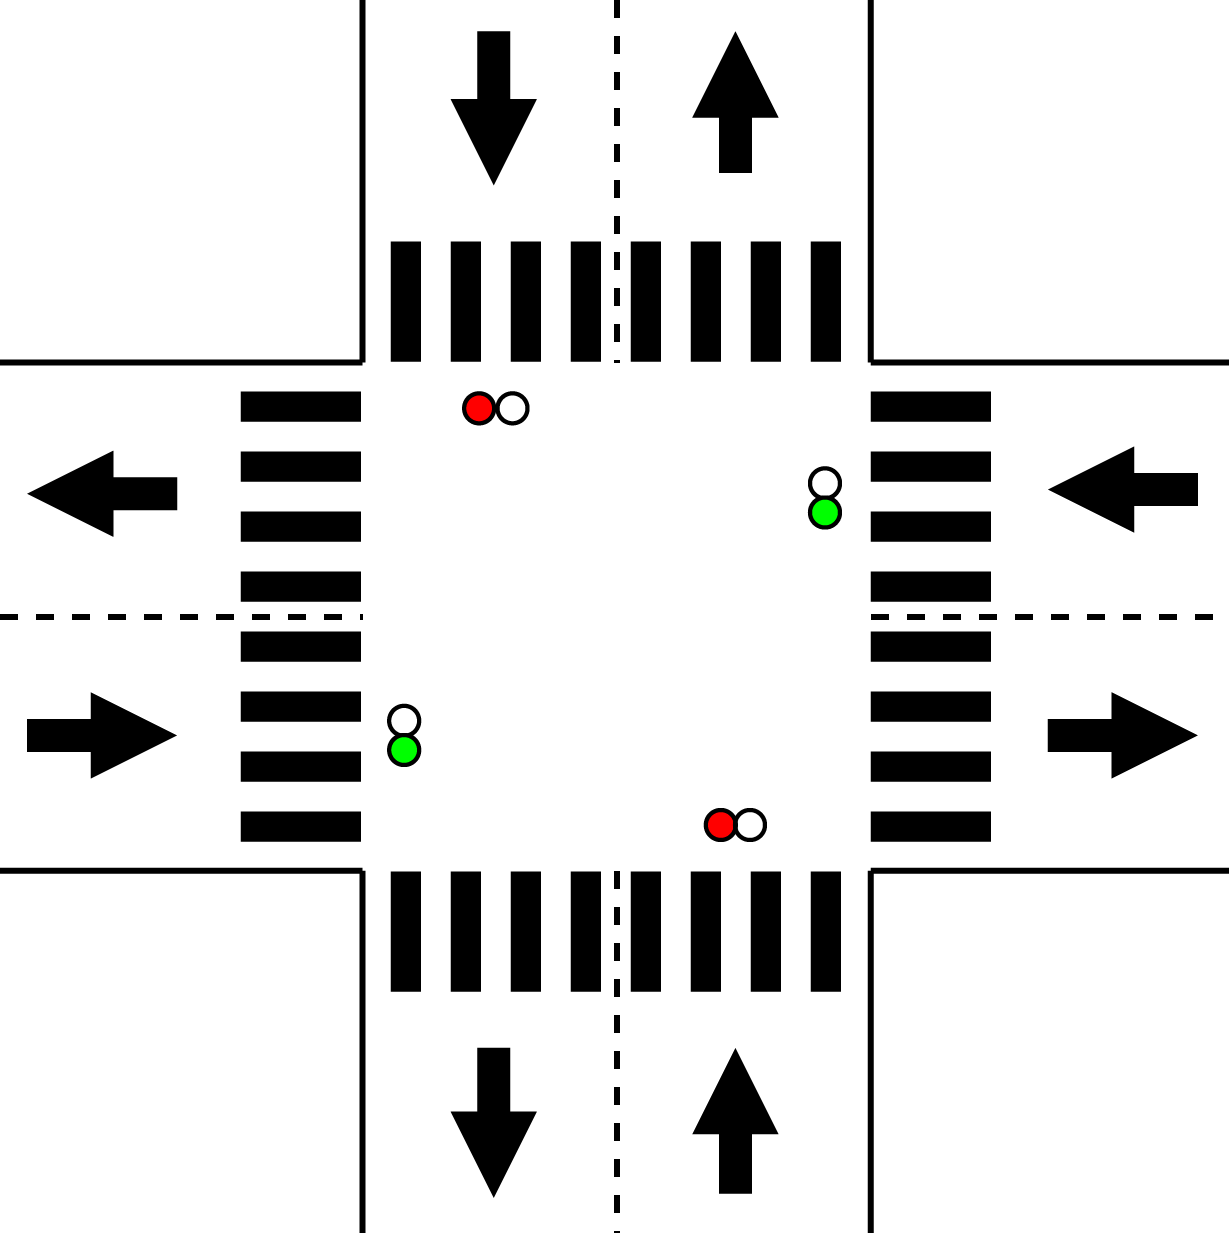
\includegraphics[width=0.5\textwidth]{picture/model/trafficlight_step1_s1.png}
    \caption{Model of the step 1}
\end{figure}

\subsubsection{Step 2: Pedestrians}
In this step, pedestrians were added and different things had to be changed to accommodate this new change. \\ 

When a pedestrians call was send by the environment, the car's traffic light that was green had to become red and the other car traffic light had to stay red. When those two traffic lights are red, the pedestrians traffic light could switch tp green. Because we also wanted fairness in our system, two assumptions were added here.
\begin{enumerate}
    \item When the pedestrians traffic light is green, we have to remember which car traffic light was previously green. This will be useful for the next assumption.
    \item We wanted fairness between the actors, even if pedestrians have the priority. The problem at the beginning was that starvation could happen if, when the pedestrians lights are green, we always switched to a specific car's traffic light. This would mean that the other car's traffic light would remain red if pedestrians are always calling. We thus added what we called a "delayed" call where, even if the pedestrians are always pressing the button, the two cars lights have to be green at least once before the pedestrians could have their lights green again. This is why the first assumption is useful, we have to remember which car's light was previously green so the cars in the other side of the crossroad don't always have to wait 2 times to be green again. \\
    As an example, if the East-West car's traffic light is green and a pedestrian pressed the button, after the pedestrians lights switch from green to red, the North-South car's traffic light is switched to green so they do not have to wait another time.
\end{enumerate}
In this step, more properties were checked. We check if, after a transition, the value of a component always reaches the enquired value. We also check, as for the first one, that certain states can never be reached in our model (all traffic lights are green for example).

\noindent In this step, we also showed thanks to PRISM that our three traffic lights were green with almost the same percentage of time. This can be seen on Figure \ref{fig:prism1}. On this graph, the X-axis represent the average time elapsed between two crosswalk calls while the Y-axis represent the number of times a traffic light is switching to the green state every T (300 in our case) units of time. What we can see is that the more time there is between the pedestrians call, the more our car traffic lights will remain green.

\begin{figure}[H]\label{fig:prism1}
  \centering
    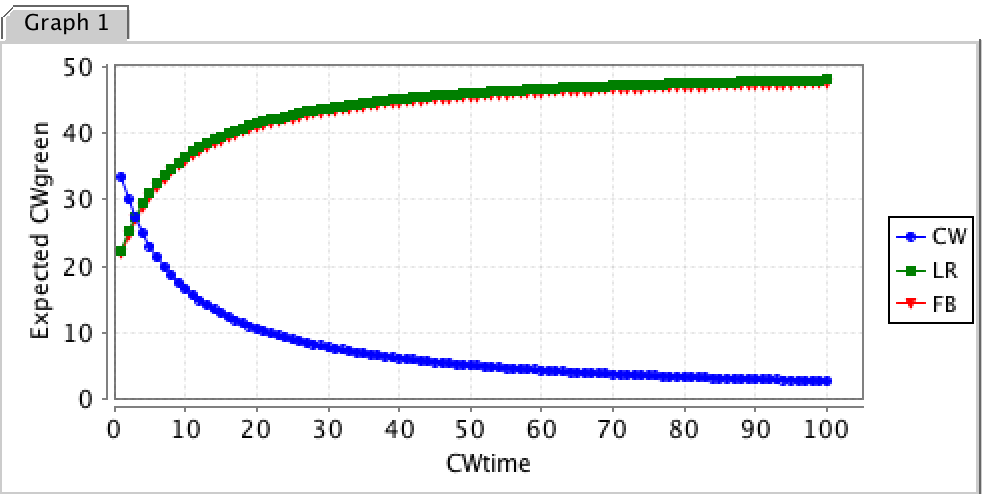
\includegraphics[width=0.5\textwidth]{picture/graphprism.png}
    \caption{Percentage of green lights between the traffic lights}
\end{figure}


\subsubsection{Step 3: Buses}
In this step, we added the buses generated by the environment. The idea here is that the buses have priority on the rest of the traffic. \\
When a bus is generated, the next traffic light that has to be green is the one of the bus. When the bus is crossing, all other lights are red because the bus will go through. The model can be seen as on Figure \ref{fig:step3bus}. \\

\begin{figure}[H]\label{fig:step3bus}
  \centering
    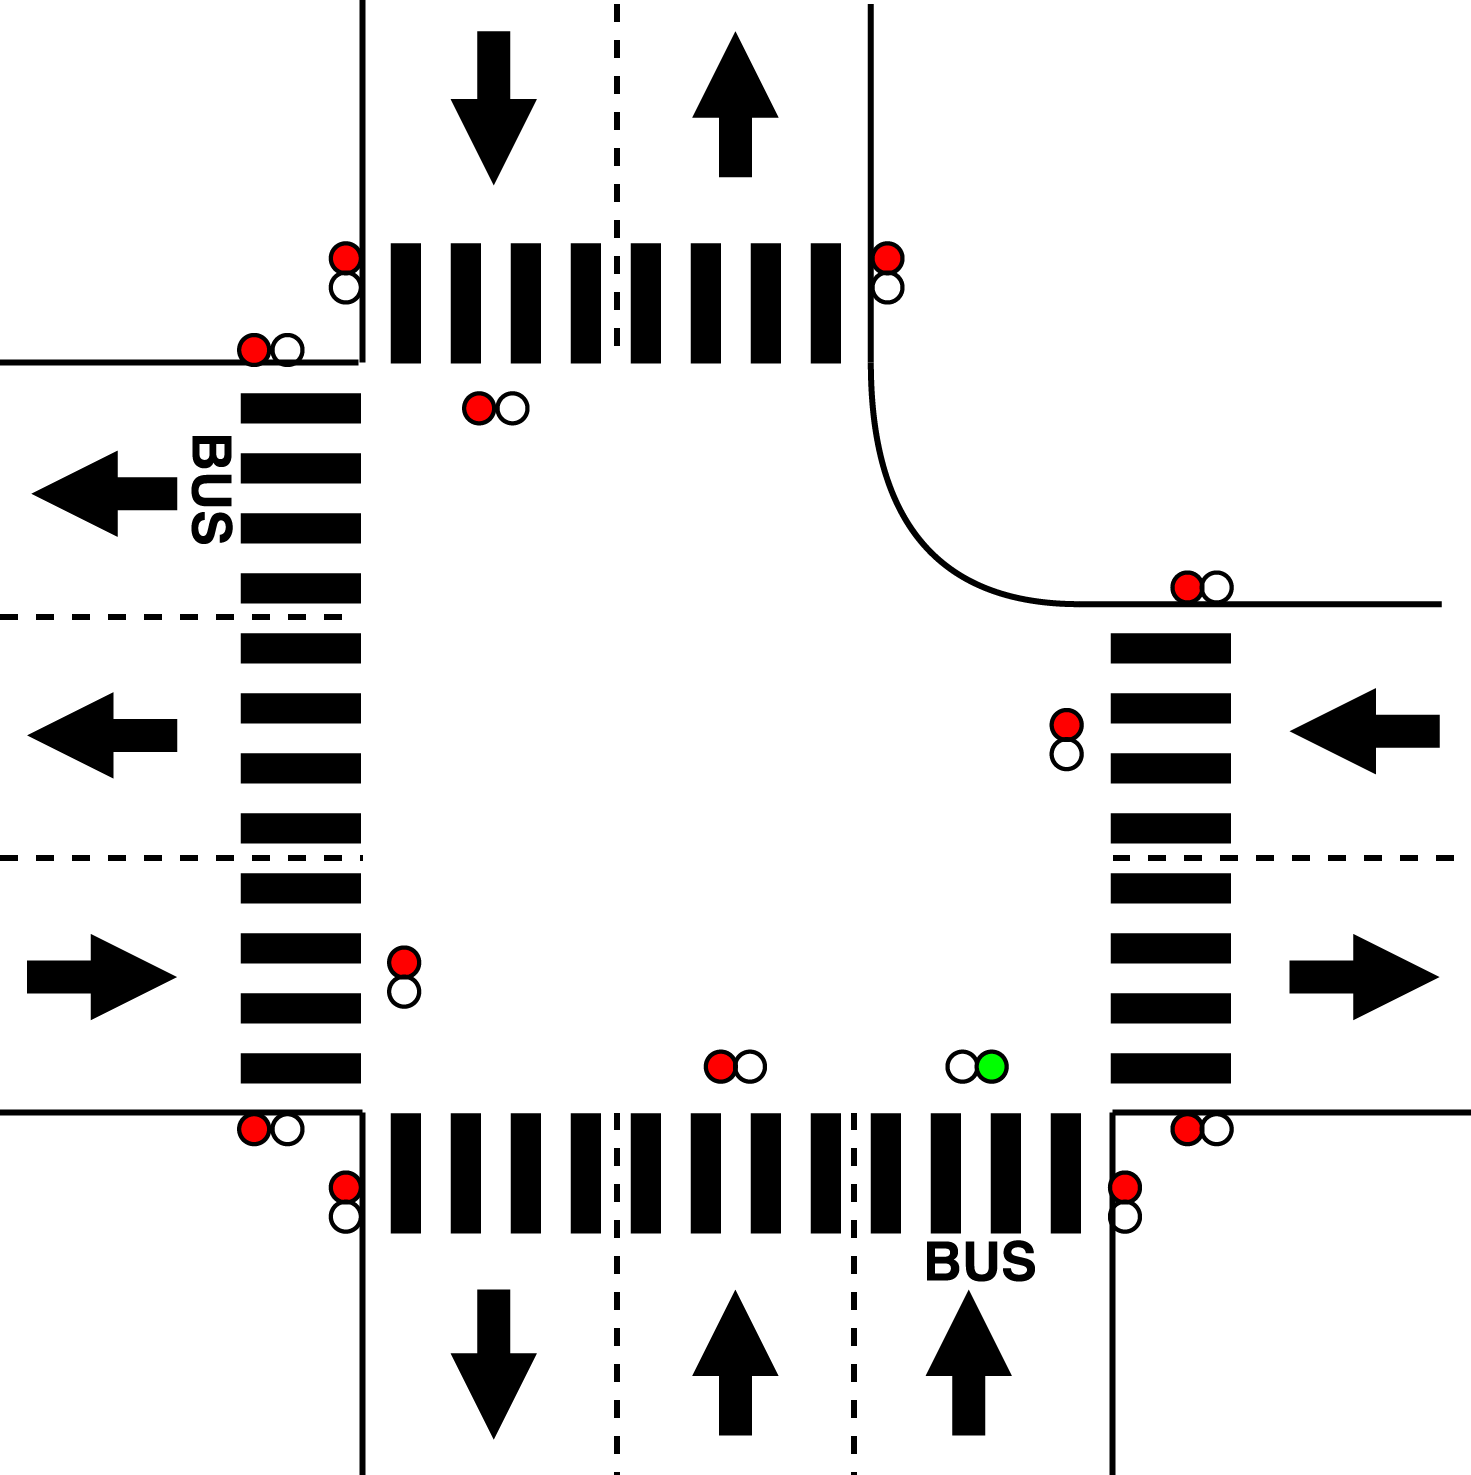
\includegraphics[width=0.5\textwidth]{picture/model/trafficlight_step3_s2.png}
    \caption{Model for the step 3}
\end{figure}


\noindent Even if the pedestrians have called to have the green lights before the bus, if a bus is generated between the call and the pedestrians green light, we will first give the green light to the bus, then the pedestrians, then the cars. This mean that the priority hierarchy is \textit{Buses-Pedestrians-Cars}. \\
This step has also been written in \textbf{PRISM}. Thanks to this probabilistic model, we obtain more specific details about our implementation. For example, we could calculate the effect of the time that has elapsed between two buses with as constant the time of a pedestrian call. We could also look at the effect of the time between two pedestrians on the green light of the bus for different time between two buses. \\

We choose to have only one dependent variable for each of the graph and fixed the value of the independent variable.
\begin{itemize}
	\item FB : the light for the car in the north-south direction,
	\item LR : the light for the car in the east-west direction,
	\item CW : the light for the pedestrians,
	\item BUS : the light for the bus.
\end{itemize}


\begin{figure}[H]\label{fig:cwfirst}
  \centering
    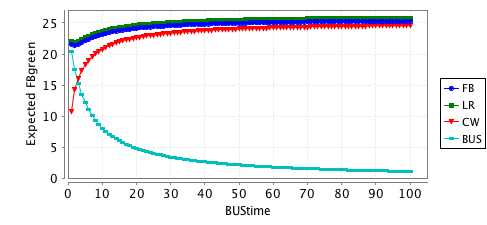
\includegraphics[width=0.5\textwidth]{picture/CWtime1.png}
    \caption{Effect of time that has elapsed between two buses with pedestrian call = 1 unit of time}
\end{figure}

\begin{figure}[H]\label{fig:cwthree}
  \centering
    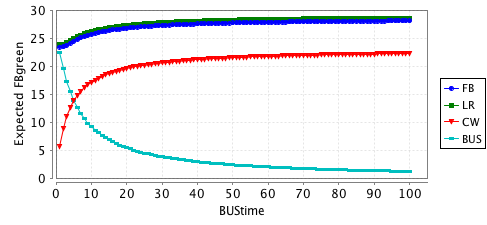
\includegraphics[width=0.5\textwidth]{picture/CWtime3.png}
    \caption{Effect of time that has elapsed between two buses with pedestrian call = 3 units of time}
\end{figure}

\begin{figure}[H]\label{fig:busbus}
  \centering
    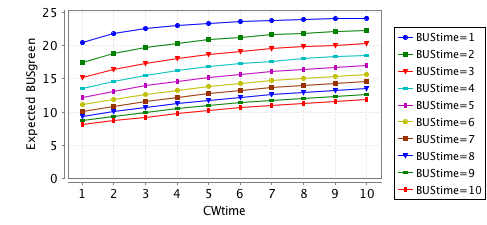
\includegraphics[width=0.5\textwidth]{picture/CWtimeOnBUS.png}
    \caption{Effect of the time between two pedestrians calls on the bus green light}
\end{figure}

Those details can be seen on Figure 4.4, 4.5 and 4.6.



\subsubsection{Step 4: Yellow Light}\label{sec:step4}
For this step, we kept the same model done in step 3 but we added a yellow light. This means that, as in the real life, our cars traffic lights will switch from green to yellow to red. \\
This is thus our final model developed in Uppaal TiGa.

\begin{figure}[H]\label{fig:step4}
  \centering
    \includegraphics[width=0.5\textwidth]{picture/model/Trafficlight_step4.png}
    \caption{Model of the step 4}
\end{figure}

\subsection{Uppaal Timed Automatons}
In order to formally model the system, we use several timed automatons from Uppaal. While some of those automatons are actors in the environment, the others are part of the controller.
The theory tells us that, when the environment is playing, we, humans, cannot decide the action that will be taken. For example, buses and pedestrians arrivals are unpredictable and uncontrollable, so they belong to the environment.
The actors which implement the solution for avoiding crashes belong to the controller. They interact with the environment in order to avoid crashes and thus they aim to find a winning strategy. \\
We will now give the implementations explanations of the environment and controller actors. In the first one, we will take a look at the pedestrians and buses generators while in the second one, we will look at our traffic light system that tries to find a winning situation (no crashes).

\subsubsection{Environment}
\paragraph{Crosswalk} \mbox{}\\
We will here talk about the mechanisms of our crosswalk generator done in our step 4 from Section \ref{sec:step4}. \\
There are several elements that can be seen on Figure 4.8.

\begin{figure}[H]\label{fig:crosswalk}
  \centering
    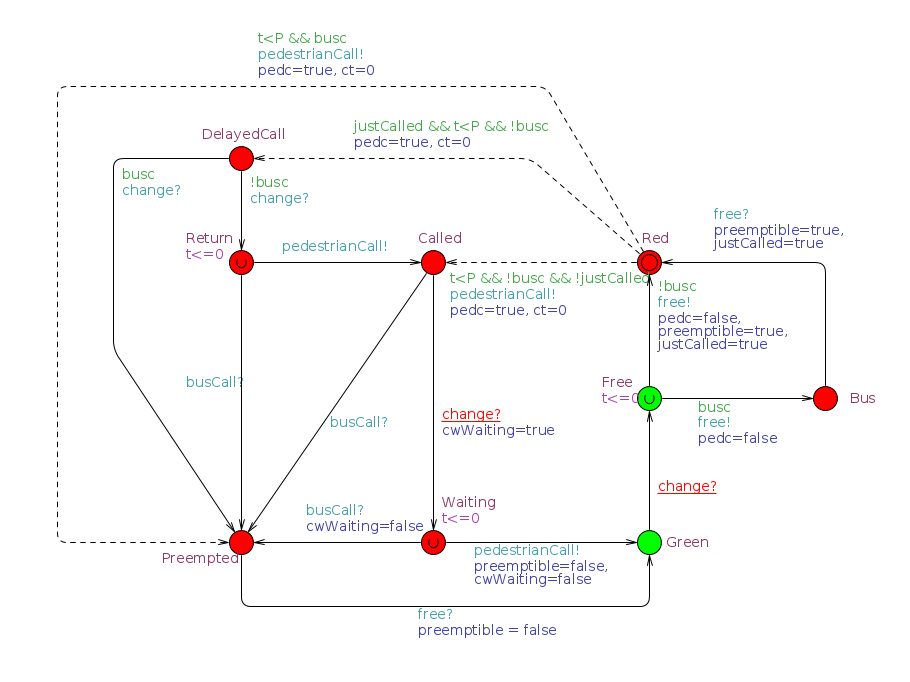
\includegraphics[width=0.9\textwidth]{picture/crosswalk.png}
    \caption{Pedestrians generator}
\end{figure}
\noindent We can see that no orange lights are present in \ref{fig:crosswalk}. Indeed, it is a pedestrians traffic lights, and like in Brussels, there is only the red and green light. We thus decided not to add an orange light for this component. \\
When the environment plays, different states can be reached. The initial state of the pedestrians lights is Red. From this state, three different destinations states are possible:
\begin{enumerate}
  \item The Preempted state: A pedestrian call has been made but there is a bus. Since they have total priority, we will first have to wait for the bus to cross the road before we can,
  \item The DelayedCall state: If there is no bus but the pedestrians already pushed the button within a certain time period in the past, we do not give them the green light immediately to stay fair,
  \item The Called state: If a call has been made and no conditions from 1 or 2 are present, we go to this state. This state means that the pedestrian will get the green light at the end of the current timer.
\end{enumerate}
At the end, every other state will reach the Preempted one after having to wait for the end of the timer. We then switch the pedestrians lights to green. After the green state, we reach a free state because, before going back to the red state, different things can happen. Indeed, a bus could arrive and since it has the priority, we will have to give him the next green light. If no bus arrived, we go back to the red state and the basic cars traffic lights will start again. 

\paragraph{Bus} \mbox{}\\
We will here talk about the mechanisms of our bus generator done in our step 4 from Section \ref{sec:step4}. \\
As for the pedestrians, four different states can be reached. We still have Preempted, DelayedCall and Called and there meaning is the same than the ones previously defined. for the pedestrians. The only difference here is that, since the bus has priority, if the pedestrians were waiting, we first have to put the bus light to green. The rest follows the same scheme as for pedestrians lights.

\begin{figure}[H]\label{fig:bus}
  \centering
    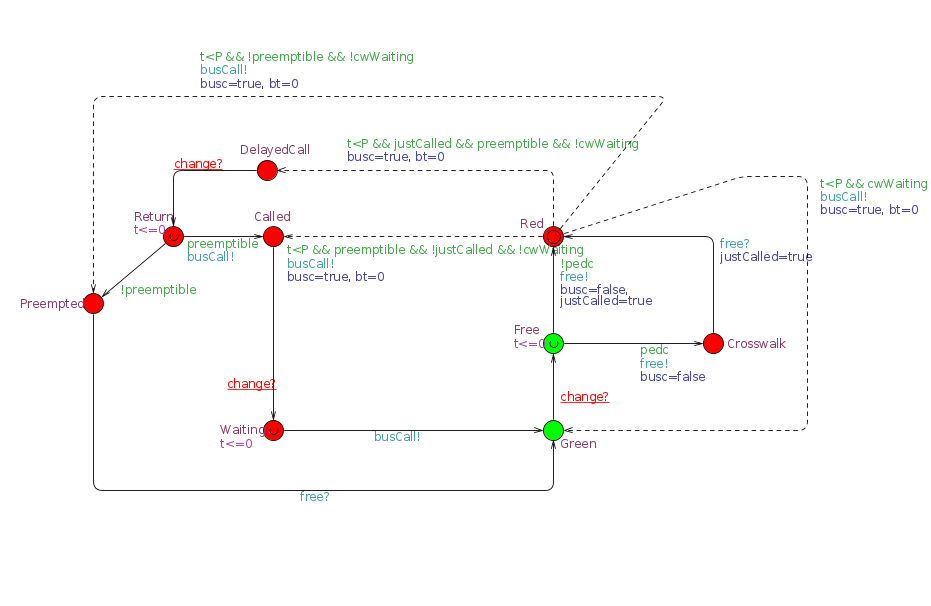
\includegraphics[width=0.9\textwidth]{picture/bus.png}
    \caption{Buses generator}
\end{figure}

\noindent Those were the two actors controlled by the environment.

\subsubsection{Controller}
\paragraph{Traffic Lights} \mbox{}\\

In this section, we will present the strategy we implemented for the controller to reach a winning strategy. \\

There are two different cars traffic lights. There is the one we called Left-Right, meaning it represents the East-West lights and the Front-Back representing the North-South crossroad. Since the idea is the same, we will just explain the Left-Right one. It just has to be kwown that the initial state for the Left-Right is the red trafic light while for the other one the initial state is the green one. \\

From the red initial state, three different states can be reached:
\begin{enumerate}
  \item If a bus has been called, the traffic light has to remain red so the bus can drive through the crosswalk. We thus reach the \textit{Bus} state.
  \item If pedestrians have pushed the button, we switch to the \textit{Crosswalk} state.
  \item If no buses or pedestrians were generated and the other cars traffic lights is switching to red, we can reach the \textit{Green} state.
\end{enumerate}

\subsection{Tested Propreties}
In this section, we will give and explain the code to formally verify that our system is correct.

\subsubsection{Liveness}
We will first give some liveness properties about our system.
\begin{enumerate}
  \item If a bus has been called, he will never have to wait indefinitely to cross the road. Since our bus can reach several states, we check for each of them if the light will be green at some point. 
  \begin{itemize}
    \item $Bus.DelayedCall --> Bus.Green$ 
    \item $Bus.Preempted --> Bus.Green$
    \item $Bus.Called --> Bus.Green$
  \end{itemize}
  \item If a pedestrian call has been made, they will never have to wait indefinitely to cross the crosswalk. Since our pedestrians can reach several states, we check for each of them if the light will be green at some point. 
  \begin{itemize}
    \item $Crosswalk.DelayedCall --> Crosswalk.Green$ 
    \item $Crosswalk.Preempted --> Crosswalk.Green$
    \item $Crosswalk.Called --> Crosswalk.Green$
  \end{itemize}
  \item No deadlock, meaning that the system will never freeze.
  \begin{itemize}
    \item \textit{A[] not deadlock}
  \end{itemize}
\end{enumerate}
Since we use Uppaal TiGa, there is not only a controller but also an environment. We thus took this into consideration and we wrote some properties about the maximum time one actor of the environment will have to wait.
\begin{enumerate}
  \item The maximum waiting time for a pedestrian is at most 3P (meaning 3 times the period we have chosen). Indeed, if he has just been called recently, he will have to wait 2P and if a bus has been called before, we have to give him the priority and wait 1P.
  \begin{itemize}
    \item \textit{A[] not( Crosswalk.Green \&\& Crosswalk.ct>4*P)}
    \item We here have to put 4P because the light will stay green until the end of the fourth green light
  \end{itemize}
  \item The maximum waiting time for a bus is at most 2P. Indeed, if he has just been called recently, he will have to wait 2P since the bus has the priority.
  \begin{itemize}
    \item \textit{A[] not( Bus.Green \&\& Bus.bt>3*P )}
    \item We here have to put 3P because the light will stay green until the end of the third green light
  \end{itemize}
  \item The cars traffich lights will be green again before 4P.
  \begin{itemize}
    \item \textit{A[] not( TrafficLightFrontBack.Green \&\& TrafficLightFrontBack.tlfbc>4*P )}
    \item \textit{A[] not( TrafficLightLeftRight.Green \&\& TrafficLightLeftRight.tllrc>4*P )}
  \end{itemize}
\end{enumerate}
\subsubsection{Safety} 
On the opposite of the first proprety we defined, the liveness one, we will here not try to find that something willeventually happen. We will here show that some events will \textbf{never} happen because if it was the case, we would reach incoherent states leading to a failure in our system. In our traffic light model, it would means that two opposite actors could cross the crossroad at the same time, leading to a crash. 
\begin{enumerate}
  \item We check that if the crosswalk light is green, no other lights can be green at the same time.
  \begin{itemize}
    \item \textit{A[] not (((Crosswalk.Green or Crosswalk.Free) and  (Bus.Green or Bus.Free)) or ((Crosswalk.Green or Crosswalk.Free) and TrafficLightFrontBack.Green) or ((Crosswalk.Green or Crosswalk.Free) and TrafficLightLeftRight.Green))}
    \item Since we consider in our model that the Free state is still a green state, we have to check for both of those states.
  \end{itemize}
  \item We check that if the bus's light is green, no other lights can be green at the same time.
  \begin{itemize}
    \item \textit{A[] not (((Bus.Green or Bus.Free) and  (Crosswalk.Green or Crosswalk.Free)) or ((Bus.Green or Bus.Free) and TrafficLightFrontBack.Green) or ((Bus.Green or Bus.Free) and TrafficLightLeftRight.Green))}
  \end{itemize}
  \item If the car FrontBack traffic light is green, no other lights can be green.
  \begin{itemize}
    \item \textit{A[] not ( (TrafficLightFrontBack.Green and (Bus.Green or Bus.Free)) or (TrafficLightFrontBack.Green and (Crosswalk.Green or Crosswalk.Free)) or (TrafficLightFrontBack.Green and TrafficLightLeftRight.Green))}
  \end{itemize}
  \item If the car LeftRight traffic light is green, no other lights can be green.
  \begin{itemize}
    \item \textit{A[] not ( (TrafficLightLeftRight.Green and (Bus.Green or Bus.Free)) or (TrafficLightLeftRight.Green and (Crosswalk.Green or Crosswalk.Free)) or (TrafficLightLeftRight.Green and TrafficLightFrontBack.Green))}
  \end{itemize}
\end{enumerate}
Thanks to those properties, we could reach a winning strategy where, even if our environment plays, everything will be under control and unfortunate situations will be avoided. In our case, it means that our crosswalk is working the way we want it to work and we were able to prove it thanks to the Verifier from Uppaal.
